\documentclass{2wa40summary}

% Used for Aart's tips
\usepackage{amsmath,amssymb}
\newcommand\inw{\mbox{int}}
\newcommand\ds{\displaystyle}
\def\diam{\text{diam}}
\parindent 0pt

\begin{document}
	\maketitle
	\thispagestyle{empty}
	\newpage
	
	\section{Inleiding}
	We nemen aan dat $d\in\naturals_+$. Met [K] wordt het boek van Kosmala aangeduid: W. Kosmala, A friendly introduction to Analysis, 2nd edition, Prentice Hall, ISBN: 0131273167
	
	Mocht je foutjes/opmerkingen/verbeteringen vinden, we zien ze graag op de \href{https://bitbucket.org/hollandpirates/analyse-2-samenvatting/issues?status=new&status=open}{issue tracker}.
	
	\section{College 15}
	\subsection{Eigenschappen van de norm}
	Voor alle $\x\in \reals^d$ en $c\in\reals$ moet gelden
	\begin{enumerate}[(i)]
		\item $|\x| \geq 0$
		\item $\abs{\x}=0 \iff \x=\zero$
		\item $|c\x|=|c||\x|$ ($|$norm$|$ = $|$absolute waarde$||$norm$|$)
	\end{enumerate}
	Als \verb#|.|# een norm is dan geldt voor alle $\x,\y\in \reals^d$ de
	\begin{enumerate}[(i)]
		\item ongelijkheid van \indx{Cauchy-Schwartz}
		\[\forall_{\x,\y \in \reals^d}: \sum_{i=1}^{d}\x_i \y_i = (\x,\y)\]
		\[|(\x,\y)| \leq |\x||\y|\]
		\item \indx{driehoeksongelijkheid}
		\[\forall_{\x,\y \in \reals^d}: |\x+\y|\leq |\x|+|\y|\]
	\end{enumerate}
	\subsection{Afstand in $\reals^d$}
	\begin{define}[Afstandsfunctie]
		Een afstandsfunctie $(\x,\y)\mapsto\dist(\x,\y)\in\reals$ heeft de eigenschap dat voor alle $\x,\y\in\reals^d$:
		\begin{align*}
		\dist(\x,\y) & \geq 0 \\
		\dist(\x,\y) & =0 \iff \x=\y \\
		\dist(\x,\y) & \leq \dist(\x,\z) + \dist(\z,\y)
		\end{align*}
	\end{define}
	De meest gebruikte afstandsfunctie \index{dist(x,y)} in $\reals^d$ is $\dist(\x,\y)\coloneqq |\x-\y|$
	
	\begin{define}[Bol]
		Laat $\x\in\reals^d$ en laat $0<r\in\reals$. Dan is de \indx{bol\ om $\x$ met straal $r$} de verzameling
		\[
		B(x,r)=\set{y \in \reals^d \: \abs{y-x}<r}.
		\]
		
	\end{define}
	\begin{define}[Inwendig punt] Zij $\x \in \reals^d$ and $A \subset \reals^d$. Dan is $\x$ een
		\indx{inwendig punt} (\textit{interior point}) van $A$
		als er $\exists_{r>0}\: B(\x,r) \subset A$.
		In dat geval heten $A$ en $B(\x,r)$ een \indx{omgeving} (\textit{neighbourhood}) van $\x$.
	\end{define}
	\begin{define}[Inwendige $\mathring{A}$, open verzameling $A$]
		Het \indx{inwendige} van $A$ is
		\[\intr A=\mathring{A}=\left\lbrace x \in A \mid \x \text{ inwendig punt van } A\right\rbrace . \]
		$A$ heet een \indx{open verzameling}\ als $A=\mathring{A}$ oftewel als
		\[
		\forall _{x \in A} \exists _{R >0}\: B(x,R) \subset A,
		\]
		oftewel elk punt van $A$ is een inwendig punt.
	\end{define}
	\begin{theorem}
		\begin{enumerate}[(1)]
			\item Zij $\left\lbrace A_\alpha \bigm| \alpha \in I \right\rbrace$ een familie van open verzamelingen $A_\alpha \subset \reals^d$, met $I$ een indexverzameling. Dan is
			\[
			\bigcup_{\alpha \in I}A_\alpha
			\]
			open.
			\item Zij $A_1,A_2,\dots,A_n \subset \reals^d$ open. Dan is
			\[
			\bigcap_{i=1}^{n}A_i
			\]
			open.
		\end{enumerate}
	\end{theorem}
	\begin{theorem}[Karakterisering voor het inwendige]
		Zij $A\subset\reals^d$. Dan is
		\item \[\intr A=\bigcup_{C \subset A, C \text{ open} }C=\bigcup \left\lbrace C \mid C \subset A \wedge C \text{ is open}\right\rbrace\]
		open. Dit volgt uit Kosmala 10.1.4.
	\end{theorem}
	\begin{define}[\indx{Rand}]
		Zij $A \subset \reals^d$. Dan
		\[\partial A\coloneqq  \reals^d\backslash (\intr A \cup \intr (\reals^d\backslash A))\]
		oftewel $x$ is een \indx{randpunt} van $A \iff x$ is geen inwendig punt van $A$ en geen inwendig punt van het complement $\reals^d\backslash A$.
		
		\textbf{Equivalente definitie.} Als $\x$ een randpunt is dan geldt voor alle $0<r\in\reals$ dat
		$B(\x,r)$ zowel een punt van $A$ als van $\reals^d \backslash A$ bevat.
	\end{define}
	\begin{lemma}
		Zij $A\subset\reals^d$.
		Elke $\x \in \reals^d$ hoort precies in 1 (exclusive or) van de drie verzamelingen
		\begin{enumerate}
			\item $\intr A$
			\item $\intr (\reals^d\backslash A)$
			\item $\partial A$.
		\end{enumerate}
	\end{lemma}
	\begin{voorbeeld}
		Zij $A = [0,1]$ dan is $\intr A=(0,1)$, $\intr (\reals^d\backslash A)=(-\infty,0)\cup(1,\infty)$
		and $\partial A = \set{0,1}$.
	\end{voorbeeld}
	
	\subsection{Stellingen uit het huiswerk}
	\begin{theorem}
		Zij $\x \in \reals^d$, $0<r\in\reals$, dan is $B(\x,r)$ open.
	\end{theorem}
	\newpage
	\section{College 16}
	\subsection{Convergentie in $\reals^d$}
	\begin{define}
		Zij $(\x\up{n}) = (x\up{1}_1,x\up{1}_2,\ldots,x\up{1}_d), (x\up{2}_1,x\up{2}_2,\ldots,x\up{2}_d), \ldots$
		een rij in $\reals^d$ en $\a =(a_1, \dots ,a_d ) \in \reals^d$. Dan heet $(\x^{(n)})$ \indx{convergent} naar $\a$ als
		\begin{enumerate}[(i)]
			\item $\abs{\x\up{n}-\a}\stackrel{n\to \infty}{\longrightarrow} 0$
			\item $\forall _{\epsilon >0} \exists _{n_0=n_0(\epsilon)} \forall _{n\geq n_0} : \abs{\x\up{n} - \a} < \epsilon$.
			\item $\forall _{\epsilon >0} \exists _{n_0=n_0(\epsilon)} \forall _{n\geq n_0} : \x\up{n} \in B(\a,\epsilon )$
		\end{enumerate}
	\end{define}		
	\begin{theorem}[Limieten voor rijtjes mogen componentsgewijs genomen worden]
		$\lim_{n\to\infty}\x\up{n}=\a \iff \lim_{n\to\infty} x\up{n}_{i} = a_i$ voor alle $i=1,\ldots ,d$.
	\end{theorem}
	
	\define[verdichtingspunt] Zij $A \subset \reals^d$. Een punt $\x \in \reals^d$ heet \indx{verdichtingspunt} van $A$ als \[\forall _{R>0}:B(\x,R)\cap  A \backslash\{\x\} \neq \emptyset.\]
	Dan $A'\coloneqq \big\{ \x \in \reals^d \bigm| \x \text{ verdichtingspunt van } A\big\}$ is de verzameling van
	alle verdichtingspunten van $A$.
	
	\lemma Zij $A \subset \reals^d$. Dan $\partial A \subset A\cup A'$.
	\define $A \subset \reals^d$ heet \indx{gesloten} als haar \underline{complement open} is.
	\valkuil Een niet open/gesloten verzameling is in het algemeen niet gesloten/open.
	Niet alle verzamelingen zijn open of gesloten. Sommige verzamelingen zoals $[0,1)$ zijn geen van beide
	en sommige andere verzamelingen zoals $\reals$ zijn zowel open als gesloten.
	
	\theorem[Karakterisering voor geslotenheid] Zij $A \subset \reals^d$. De volgende beweringen zijn equivalent:
	\begin{enumerate}[(i)]
		\item $A$ gesloten
		\item $A'\subset A$
		\item $\partial A \subset A$
		%\item voor elke convergente rij in $A$ ligt de limiet in $A$. (limiet convergente rij blijft in $A$)
		\item voor elke convergente rij $(\x\up{n})\to\x$ met $\set{\x\up{n}}\subset A$ geldt dat de limiet $\x\in A$.% (limiet convergente rij blijft in $A$)
	\end{enumerate}
	
	\theorem $\left[\text{K}\right]$ 10.1.6
	\begin{enumerate}[(i)]
		\item Zij $\big\{ A_\alpha \bigm| \alpha \in I \big\}$ een familie gesloten verzamelingen $A_\alpha \subset \reals^d$ met $I$ een indexverzameling. Dan $\bigcap_{\alpha \in I}A_\alpha$ gesloten.
		\item Zij $A_1, \dots ,A_n$ gesloten. Dan $\bigcup_{i=1}^n A_i$ gesloten.
	\end{enumerate}
	
	\define[afsluiting] Zij $A \subset \reals^d$. De verzameling $\overline{A}\coloneqq  \reals^d \backslash (\intr (\reals^d \backslash A))$ heet de \indx{afsluiting} (\textit{closure}) van $A$.
	\theorem[Karakterisering  van de afsluiting]
	Zij $A \subset \reals^d$. Dan
	\[\overline{A}= A \cup \partial A = A \cup A'= \big\{\z \in \reals^d \bigm| \exists _{\text{rij } (\x\up{n}) \text{ in } A \text{ met } \x\up{n} \to \z} \big\}.\]
	
	\subsection{Stellingen uit het huiswerk}
	\theorem Zij $(\x\up{n})$ een rij in $\reals^d, \a \in \reals^d$. Dan $\x\up{n}\to \a \implies |\x\up{n}|\to |\a|.$
	\theorem Zij $\z \in \reals^d, A \subset \reals^d, A \neq \emptyset, \text{dist}(\z,A) \coloneqq  \text{inf}_{\x\in A}|\x-\z|$.
	Dan $\overline{A}=\big\{\z\in \reals^d \bigm| \text{dist}(\z,A)=0\big\}$.
	\newpage
	\section{College 17}
	\subsection{Compacte verzamelingen in $\reals^d$}
	\define Een verzameling $A\subset\reals^d$ heet \indx{begrensd} als \[\exists _{R>0}: A \subset B(\zero,R)\]
	\[\exists _{R>0} \forall _{\x\in A}: \abs{\x}<R.\]
	
	\theorem $\left[\text{K}\right]$ 10.1.7 (andere formulering)
	Zij $A \subset \reals^d$. De volgende beweringen zijn equivalent:
	\begin{enumerate}[(i)]
		\item Elke rij $\x\up{n}$ in $A$ heeft een convergente deelrij met limiet $\x^* \in A$.
		\item $A$ begrensd en gesloten
	\end{enumerate}
	
	\define[overdekking] Zij $A \subset \reals^d$. Een familie $\big\{A_\alpha \bigm| \alpha \in I \big\}$ van verzamelingen $A_\alpha \subset \reals^d$ heet een \indx{overdekking} (\textit{cover, covering}) van $A$ als \[A \subset \bigcup_{\alpha \in I}A_\alpha.\]
	
	\begin{itemize}
		\item Een overdekking $\big\{ A_\alpha \bigm| \alpha \in I \big\}$ heet \textit{open} als alle $A_\alpha$ open zijn in $\reals^d$.
		\item Een overdekking $B\coloneqq \big\{ A_\beta \bigm| \beta \in J\big\}$ heet een \indx{deeloverdekking} van $A\coloneqq \big\{ A_\alpha \bigm| \alpha \in I \big\}$ als $B \subset A$.
	\end{itemize}
	
	\define[compact] $K \subset \reals^d$ heet \indx{compact} als elke open overdekking van $K$ een eindige deeloverdekking bevat.
	\valkuil Niet-lege open verzamelingen zijn NOOIT compact.
	
	\theorem[Heine-Borel]
	Zij $K \subset \reals^d$. Dan \[K \text{ compact}\iff K \text{ begrensd en gesloten.}\]
	
	\theorem Zij $A,B$ gesloten, niet leeg, $A\cap B = \emptyset$, $A$ compact.
	Dan $\text{dist}(A,B) = \text{inf}\big\{ |a-b| \bigm| a \in A, b \in B \big\} > 0$.
	\define[relatief compact] $A \subset \reals^d$ heet \indx{relatief compact} $\iff \overline{A}$ compact.
	
	\subsection{Stellingen uit het huiswerk}
	\theorem Zij $A \subset \reals^d$. Equivalente beweringen:
	\begin{enumerate}[(i)]
		\item $A$ is begrensd
		\item $\exists _{x \in \reals^d} \exists _{R>0}: A \subset B(x,R)$
		\item $\forall _{x \in \reals^d} \exists _{R>0}: A \subset B(x,R)$
		\item De verzamelingen $\{ x_i | x \in A \}, i=1,\dots,d$ zijn begrensde deelverzamelingen van $\reals$
		\item De verzameling $\big\{|x-y| \bigm| x,y \in A \big\}$ is begrensd.
	\end{enumerate}
	
	\theorem Zij $A \subset \reals^d$. Dan \[A \text{ begrensd} \iff \overline{A} \text{ begrensd} \iff \overline{A}\text{ compact}.\]
	
	\define[Cauchyrij] Een \indx{Cauchyrij} $(\x\up{n})$ in $\reals^d$ is een rij waarvoor geldt dat\[\forall _{\epsilon >0} \exists _{n_0=n_0(\epsilon )\in \naturals}\forall _{n,m \geq n_0}: |\x\up{n}-\x\up{m}| < \epsilon.\]
	\theorem Elke Cauchyrij $(\x\up{n})\subset\reals^d$ is convergent in $\reals^d$.
	
	\newpage
	\section{College 18}
	\subsection{Functies $\reals^d \to \reals$: limieten en continu\"{\i}teit}
	\define[Limiet] Zij $D \subset \reals^d, f\: D\to \reals, \a \in D', L\in\reals$.
	De \indx{limiet} (\textit{limit}) van $f(\x)$ voor $\x\to\a$:
	\[ \lim_{\x\to \a}f(x)=L \iff \left( \forall _{\epsilon >0} \exists _{\delta >0} \forall _{\x \in D}: 0<|\x-\a|<\delta \implies |f(\x)-L|<\epsilon \right). \]
	
	\theorem Zij $D \subset \reals^d, f\: D\to \reals, \a \in D', L \in \reals$. Dan geldt
	\[ \lim_{\x \to \a} f(\x)=L \iff \text{voor elke rij } (\x\up{n}) \text{ in } D\backslash\{\a\} \text{ met } \x\up{n}\to \a \text{ geldt } f(\x\up{n}) \to L.\]
	
	\opm ($\left[\text{K}\right]$ 10.2.5) De limietstellingen zijn analoog aan 1D.
	
	\define[\indx{continu te $\a$ voor $f$}] Zij $D \subset \reals^d, \a\in D\cap D',f\: D\to \reals$. $f$ heet continu te $\a$ als \[\lim_{\x\to \a}f(\x)=f(\a) \text{ oftewel als}\]
	\[\forall _{\epsilon >0} \exists _{\delta >0}: \x \in B(\a,\delta)\cap D \implies |f(\x)-f(\a)|<\epsilon.\]
	
	\theorem ($\left[\text{K}\right]$ 10.2.7)
	$f$ continu te $\a\iff ($voor elke rij $(\x\up{n})$ in $D: \x\up{n}\to \a \implies f(\x\up{n}) \to f(\a) ).$
	
	\theorem Betreffende de continu\"iteit van samengestelde functies. Zij
	$D \subset \reals^d, \a \in D\cap D', f,g\: D\to \reals$, beide continu te $\a$ en $\zero \not \in R(g)$.
	Dan zijn
	\begin{itemize}
		\item $f+g$
		\item $fg$
		\item $\dfrac{f}{g}$
	\end{itemize}
	continu te $\a$.
	
	\define[\indx{Vectorwaardige functies}]
	Zij $D \subset \reals^d, \f\: D\to \reals^m, m \in \naturals_+$. Dat wil zeggen
	\[\f(\x)=\f(x_1,\dots , x_d) =
	\begin{bmatrix}
	f_1(x_1,\dots , x_d) \\
	\vdots \\
	f_m(x_1,\dots , x_d) \\
	\end{bmatrix}\in\reals^m, \qquad f_i\:D\to \reals.\]
	
	\theorem[Limieten voor functies mogen componentsgewijs genomen worden] Zij $\a \in D'$.
	\begin{align*}
	\lim_{\x\to\a}\f(\x)=L \in \reals^m  &\iff \lim_{\x\to\a}f_i(\x)=L_i \ (i=1,\ldots ,m) \\
	&\iff \forall _{\epsilon >0} \exists _{\delta >0}: 0<|\x-\a|<\delta, \x\in D \implies \abs{\f(\x)-L}<\epsilon.
	\end{align*}
	
	\define[\indx{continu te $\a$ voor $\f$}] Zij $D \subset \reals^d$, $\a \in D \cap D'$ en $\f\: D \to \reals^m$ een vectorwaardige functie.
	Dan is $\f$ continu te $\a$ als:
	\begin{align*}
	\forall _{\epsilon >0} \exists _{\delta >0}: \x\in B(\a,\delta)\backslash\set{\a} &\implies |\f(\x)-\f(\a)|<\epsilon \\
	&\implies \f(\x) \in B(\f(\a),\epsilon).
	\end{align*}
	
	\define De volgende beweringen zijn equivalent: Zij $D\subset\reals^d$ het domein van $\f$.
	\begin{enumerate}[(i)]
		\item $\f$ continu te $\a$
		\item $f_i$ continu te $\a$ voor $i=1,\ldots,m$
		\item voor elke rij $(\x\up{n})$ in $D$ met $\x\up{n}\to\a$ geldt $f_i(\x\up{n}) \to f_i(\a),\quad i=1,\ldots,m$
		\item voor elke rij $(\x\up{n})$ in $D$ met $\x\up{n}\to\a$ geldt $\f(\x\up{n})\to\f(\a)$
	\end{enumerate}
	
	\define[\indx{continu te $D\subset\reals^d$ voor $\f$}]
	Laat $D \subset \reals^d$. Dan is $\f\: D \to \reals^m$ continu $\iff$ $\f$ is continu te elke $\a\in D\cap D'$.
	\opm Zij $\f\: D\to \reals^m$ continu en $(\x\up{n})$ een rij in $D$ met $\x^{(n)} \to \x^* \in D$.
	Dan $\f(\x\up{n}) \to \f(\x^*).$
	
	\newpage
	\section{College 19}
	\subsection{Eigenschappen van continue functies in $\reals^d$}
	\begin{theorem}[continue functies en compacte verzamelingen]
		Zij $D \subset \reals^d$ compact, $\f\: D\to\reals^m$ continu. Dan is
		\begin{enumerate}[(1)]
			\item $\f(D)$ compact (continue functies beelden compacte verzamelingen af op compacte verzamelingen)
			\item $\f$ \indx{uniform continu}, oftewel
			\[\forall_{\epsilon > 0} \exists_{\delta = \delta(\epsilon)}\forall_{\x,\z\in D}:
			\abs{\x-\z}<\delta \implies |\f(\x)-\f(\z)|<\epsilon.
			\]
		\end{enumerate}
		\opm Merk op dat bij uniforme continu\"iteit $\delta$ niet af mag hangen van $\x$ of $\z$, maar er moet zo'n $\delta$ te vinden zijn voor de hele verzameling.
	\end{theorem}
	
	\gevolg[continue functies op compacte verzamelingen nemen een minimum en maximum aan]
	Stel $f\: D\subset~\reals\to~\reals$ is continu
	en $D$ is compact. Dan is $f$ begrensd en $\exists_{\x^* \in D}:f(\x^*)=\max_{\x\in D}\set{f(\x)}$.
	
	\subsection{Compositie van continue functies}
	\theorem Zij $\f\: D\subset\reals^d\to \reals^k$ continu, $\g\: E\subset\reals^k\to \reals^l$ continu en $\f(D) \subset E$. Dan $\g \circ \f\: D\to \reals^l$ continu.
	
	\subsection{De vastepuntstelling van Banach}
	\begin{theorem}
		Zij $D \subset \reals^d$.
		Een afbeelding $\F\: D \to \reals^d$ heet \indx{contraherend} (\textit{contracting}) als
		\[\forall _{\x,\y\in D}\exists _{q \in (0,1)}:\abs{\F(\x)-\F(\y)}_{\reals^d} \leq q\abs{\x-\y}_{\reals^d}. \]
	\end{theorem}
	
	
	\gevolg $\F$ contraherend op $D\subset\reals^d\implies\F$ continu op $D$.
	
	
	\begin{define}[iteratierij]
		Stel $\F\: D\to D$, oftewel $\F(D) \subset D$. Kies \indx{startbenadering} $\x\up{0} \in D$.
		Dan bestaat de rij $(\x\up{n})$ gedefinieerd door
		\[
		\x\up{n+1} \coloneqq  \F(\x\up{n})
		\]
		en heet~\indx{iteratierij}.
	\end{define}
	
	
	%			Stel $F:D\to D$, oftewel $F(D) \subset D$. Elke rij $(x_n)$ met $F(x_n) = x_{n+1}$ heet \textbf{iteratierij} (met startvoorwaarde $x_0 \in D$).
	
	\theorem[vastepuntstelling van Banach\index{Banach, vastepuntstelling van}]
	Zij $D \subset \reals^d, \F\: D\to \reals^d$. Veronderstel
	\begin{enumerate}[(i)]
		\item $D$ gesloten
		\item $\F\: D \to D$ ($\F(D) \subset D$)
		\item $\F$ contraherend
	\end{enumerate}
	Dan
	\begin{enumerate}[(1)]
		\item $\exists!_{\x^* \in D}$ met $\F(\x^*)=\x^*$.
		\item Voor elke $\x_0 \in D$ convergeert de iteratierij naar $\x^*$.
	\end{enumerate}
	
	\subsection{Differentieerbare functies van meerdere variabelen}
	\subsubsection{Parti\"ele functies en parti\"ele afgeleiden}
	
	\begin{define}[parti\"ele functies]
		Zij $D \subset \reals^2$ open. $F\: D \to \reals$, $(a,b) \in D$.
		De functies
		\begin{enumerate}
			\item $p_b\: S_b \to \reals$, $p_b(x)\coloneqq f(x,b)$
			\item $q_a\: T_a \to \reals$, $q_a(y)\coloneqq f(a,y)$
		\end{enumerate}
		heten \indx{parti\"ele functies}.
		Alternatieve notatie:
		\begin{enumerate}
			\item $p_b\coloneqq f(\cdot, b)$
			\item $q_a\coloneqq f(a,\cdot)$
		\end{enumerate}
		
	\end{define}
	\red{Let op: $S_b$ en $T_a$ zijn niet gedefinieerd. Voor de hand ligt $S_b = \set{b\in\reals\:(x,b)\in D}$.}
	
	\begin{define}[parti\"eel differentieerbaar]
		Als $p_b/q_a$ differentieerbaar is in $x=a/y=b$ dan heet $f$ \indx{partieel differentieerbaar} naar $x/y$ in $(a,b)$
		en defini\"eren we
		\begin{itemize}
			\item $\partial_x f(a,b) \coloneqq  p_b'(a)$
			\item $\partial_y f(a,b) \coloneqq  q_a'(b) $
		\end{itemize}
		
	\end{define}
	
	\begin{gevolg}[parti\"eel differentieerbaar (2)]
		
		Deze definitie is equivalent met
		\begin{itemize}
			\item $\displaystyle\partial_x f(a,b)=\lim_{h \to 0} \frac{f(a+h,b)-f(a,b)}{h}$
			\item $\displaystyle\partial_y f(a,b)=\lim_{k \to 0} \frac{f(a,b+k)-f(a,b)}{k}$
		\end{itemize}
		
	\end{gevolg}
	
	
	
	\subsection{Stellingen uit het huiswerk}
	\theorem Zij $D \subset \reals^d$. Een functie $\f\: D \to \reals^m$ heet \indx{Lipschitz-continu} als er een $L>0$ is zodanig dat
	\[\forall _{\x,\y \in D}: |\f(\x)-\f(\y)|_{\reals^m} \leq L|\x-\y|_{\reals^d}.\]
	Elke Lipschitz-continue functie is uniform continu op $D$.
	\newpage
	\section{College 20}
	\subsection{Hogere orde parti\"ele afgeleiden}
	\define[inductief] Parti\"ele afgeleiden van orde $k+1$ zijn de parti\"ele afgeleiden van de parti\"ele afgeleiden van orde $k$.
	\theorem[Schwarz of Clairaut] Neem $D \subset \reals^d$ open. Als $f\: D \to \reals$ twee keer continu partieel differentieerbaar in $D$ is
        dan geldt $\partial_i \partial_j f(\a) = \partial_j \partial_i f(\a) \quad i,j=1,\dots ,d$ voor alle $\a \in D$.
	\subsection{Totale differentieerbaarheid}
	\define [Fr\'echet-differentieerbaar] Zij $D \subset \reals^d$ open en $\a \in D$. Als
 er is een lineaire afbeelding $L_{\a}\:\reals^d \to~\reals$ bestaat zodanig dat
	\[f(\a+\h)=f(\a)+ L_{\a} \h +\mathrm{o}(\abs{\h})\iff\lim_{\h\to0}\frac{\abs{f(\a+\h)-f(\a)-L_{\a} \h}}{\abs{\h}} = 0\]
 dan heet $f\: D \to \reals$ \indx{differentieerbaar} (\indx{totaal differentieerbaar}, \indx{Fr\'echet-differentieerbaar}) te $\a \in D$
	en heet $L_{\a}$ \textbf{afgeleide van} $f$ \textbf{te} $\a$.
	\nota $L_{\a} = f'(\a) = [\partial_1 f,\ldots,\partial_m f](\a)\in\reals^{1\times d}$
	\subsection{De gradi\"ent}
	\theorem[linearisering, gradi\"ent en parti\"ele afgeleide] Zij $D \subset \reals^d$ open, $\f\:  D \to \reals^d$, differentieerbaar te $\a \in D$. Dan $f$ partieel differentieerbaar te $\a$, en
\[\nabla \f(\a)= \begin{bmatrix}
\partial_1 \f(\a) \\
\vdots \\
\partial_d \f(\a)
\end{bmatrix} = \f' \fallingdotseq \f^\prime (\a)^{T}\in\reals^{d\times 1}.
\]

	\theorem Zij $D \subset \reals^d$, $D$ open. Als $f\: D \to \reals$ differentieerbaar te $\a \in D$ dan is $f$ ook continu te $\a$.
      		
	\define De functie $ p\:  \reals^d \to \reals $ gegeven door \[p(x)=f(a)+f'(a)(x-a)\] heet \textbf{lineaire approximatie} van $ f $ in/rond $ a $.
	\newpage	
	\section{College 21}
		Zij $D \subset \reals^d$ open, $\a\in D$, $f\: D \to \reals$.

%\[
%\begin{array}{rcl}
%f \text{\textbf{totaal differentieerbaar te }} \a &\implies
%f \text{\textbf{partieel differentieerbaar te }} \a \\
%\hline
%f \text{\textbf{totaal differentieerbaar te }} \a &\leftarrow
%{f \text{\textbf{partieel differentieerbaar te }} \a \text{ en}\atop \text{\textbf{alle parti\"ele afgeleide continu te } \a}}\\
%\end{array}
%\]
		
    	\begin{tabular}{l p{3cm} r}
    		\textbf{$f$ partieel differentieerbaar bij $a$} & & \textbf{$f$ totaal differentieerbaar bij $a$} \\
    		& \center $\centernot \implies$ & \\
 			$\partial_i f(a)= \lim_{h \to 0} \frac{f(a+he_i)-f(a)}{h}$ bestaat & \center $\Longleftarrow$ & $\frac{f(a+h)-f(a)-f'(a)[h]}{|h|}\stackrel{h \to 0}{\to} 0$ \\
 			& \center $\implies$ & \\
 			& voorwaarde: part afg bestaan en zijn continu in omgeving $a$& \\   		
		\end{tabular}
		\theorem[K 10.4.5] Zij $D\subset\reals^d$, $f\: D\to\reals$ part differentieerbaar in een omgeving van $\a \in \intr D$ en $\partial_i f \quad i=1,\dots ,d$ continu te $\a$. Dan $f$ differentieerbaar in $\a$.
		
		\subsection{Richtingsafgeleiden}
\begin{define}[Richtingsvector]
Een vector $\u\in\reals^d$ met $\abs{\u}=1$ heet \indx{richtingsvector}.
\end{define}
\begin{define}[Richtingsafgeleide]
			Zij $D \subset \reals^d$ open, $\a \in D$, $\u \in \reals^d$ een richtingsvector. Zij $f\: D \to \reals$ differentieerbaar te $a$.
Dan is de \indx{richtingsafgeleide} van $f$ in de richting van $\u$ gegeven door
			\begin{equation} \label{eq:rafg}
			   	  		D_{\u} f(\a) \coloneqq  \lim_{t \to 0} \dfrac{f(\a+t\u) - f(\a)}{t}
			\end{equation}
			Speciale gevallen:
\[\u=\e_i \implies D_{\e_i}f(\a)=\partial_i f(\a)\].
\end{define}
\begin{theorem} [K 10.5.2]
Veronderstel de situatie zoals in de definitie hierboven. Dan geldt
			\[D_{\u} f(\a)= \lim_{t \to 0} \dfrac{f(\a+t\u) - f(\a)}{t}=(\nabla f(\a),\u).\]  	  	
\end{theorem}
			\gevolg Stel $\nabla f(\a) \neq 0$. De functie $f \Longunderstack{\text{ stijgt }\cr \text{ daalt }}$ bij $\a$ het sterkst in de richting $\ds\pm \dfrac{\nabla f(\a)}{\abs{\nabla f(\a)}}$.	
			
		\subsection{Differentieerbaarheid van vectorwaardige functies, Jacobimatrix}
			Zij $D \subset \mathbb{R}^d$ open, $a \in D. f\:  D \to \mathbb{R}^m$. $f$ is differentieerbaar in $a$ als er een lineaire afbeelding $L_a \: \mathbb{R}^n \to \mathbb{R}^m$ bestaat zodanig dat \[f(x)=f(a)+L_a (x-a) + r(x) \qquad \lim_{x \to 0} \frac{r(x)}{|x-a|} =0 \quad\text{ (lim in } \mathbb{R}^m \text{!)}\]
			Co\"ordinaten: $\underline{f}(x_1,\dots ,x_n)=\begin{bmatrix}
				f_1 (x_1, \dots ,x_n) \\
				\vdots \\
				f_m (x_1, \dots ,x_n)
			\end{bmatrix}$
			\theorem[en definitie] Situatie als beschreven. $f$ differentieerbaar in $a \implies$ alle part afg $\frac{\partial f_i}{\partial x_j}(a)$ bestaan, en
			\[[L_a] = \begin{bmatrix}
				\partial_1 f_1 (a) & \partial_2 f_1 (a) & \dots &\partial_n f_1 (a) \\
				\vdots & & & \vdots \\
				\partial_1 f_m (a) & \partial_1 f_m (a) & \dots &\partial_n f_m (a)
			\end{bmatrix} \qquad \textbf{\indx{Jacobimatrix}}\]
			Dat wil zeggen: $[L_a]_{ij}=\frac{\partial f_i}{\partial x_j}(a)$.
			\nota $\frac{\partial f_i}{\partial x_j}(a)$, $\frac{\partial (f_1,\dots,f_m)}{\partial (x_1,\dots,x_n)}(a)$, $ Df(a) $.
			
			Om te onthouden:
			\[ \frac{\partial f}{\partial x} = \begin{bmatrix}
			\dots & (\nabla f_1)^\top & \dots \\
			& \vdots & \\
			\dots & (\nabla f_m)^\top & \dots
			\end{bmatrix} =
			\begin{bmatrix}
			\vdots & & \vdots \\
			\partial_1 \underline{f} & \dots & \partial_n \underline{f} \\
			\vdots & & \vdots
			\end{bmatrix}\]
			
		\subsection{Stellingen uit het huiswerk}
			\theorem Zij $ D \subseteq \mathbb{R}^d $ open, $ f\:  D \to \mathbb{R}^m $ met co\"ordinaatvoorstelling $ f=(f_1,\dots,f_m) $ waarbij $ f_i \:  D \to \mathbb{R} $. Zij $ a \in D $. Dan
			\begin{enumerate}[(1)]
				\item $ f $ differentieerbaar in $ a \iff $ alle $ f_i $ differentieerbaar in $ a $.
				\item Alle eerste orde part afg $ \partial_j f_i $ bestaan in een omgeving van $ a $ en zijn continu bij $ a $, dan is $ f $ differentieerbaar bij $ a $.
			\end{enumerate}
			\theorem Zij $ A $ een $ (m,n) $-matrix en zij $ f\: \mathbb{R}^n \to \mathbb{R}^m $ gegeven door $ f(x)=Ax $. Dan $ f $ differentieerbaar op $ \mathbb{R}^n $ en $ Df(x) = A $.
			
	\newpage
	\section{College 22}
		\subsection{Kettingregel}
			\theorem Zij $g\: D \to E$ differentieerbaar in $a \in D$, $D \subseteq \reals^n$ open, $f\: E \to \reals^k$ differentieerbaar in $g(a)$, $g(D) \subseteq E$, $E \subseteq \reals^m$ open.
			
			Dan $f\circ g\: D\to \reals^k$ is differentieerbaar bij $a$, en \[ D(f \circ g)(a) = Df(g(a))\circ Dg(a). \]
			
			\begin{voorbeeld}[Onthouden]
				Zij $f \: \reals^2 \to \reals$, differentieerbaar. Zij $g(t) = \vvec{x(t)\\y(t)}$. Dan
				\[ 
				(f \circ g)(t) = f(x(t),y(t)).
				\]
				Dan volgt uit de kettingregel dat $ f \circ g $ differentieerbaar is en $ \frac{df}{dt} = \frac{\partial_f}{\partial_x}\cdot\frac{\partial_x}{\partial_t} + \frac{\partial_f}{\partial_y} \cdot \frac{\partial_y}{\partial_t}$. Dit is te onthouden door in onderstaande boom alle paden van $f$ naar $t$ te volgen.
				
				\Tree[.f 
						[.x
							[.t ] 
						]
						[.y
							[.t ]
						]
					]
				
				
			\end{voorbeeld}
			
			\gevolg en \textbf{definitie.} Zij $f\: D \subset \reals^d \to \reals$, $c \in \reals$. 
			
			$S_c = \left\{ x\in D \middle| f(x)=c \right\}$ heet een \textbf{niveaulijn, niveauoppervlak, niveauverzameling}.
			
			Zij $I$ een interval, $g\:  I\to S_c$ differentieerbaar, dan $f(g(t))=c \forall_{t \in I}$.
			
			\opm Kettingregel $\implies (\nabla f(g(t)),g'(t)) = 0$, ofwel de gradi\"ent $\bot$ raakvlak, niveauverzameling, niveaulijnen.
			
		\subsection{Kettingregel en richtingsafgeleiden}
			
			\define \textbf{Richtingsafgeleide} (Ook als $|v|\neq 1$)
			Zij $f$ voldoende vaak continu differentieerbaar, $v=(v_1,...,v_d) \in \reals^d$ vast.
			
			Dan is \[ D_v^2 f = (v_1 \partial_1 + ... + v_d \partial_d)(v_1 \partial_1 + ... + v_d \partial_d)f = \sum_{i,j=1}^{d} v_i v_j \partial_{ij}f \]
			
			\[ D_v^k f = \sum_{i_1,...,i_k=1}^{d} v_{{i_1},...,v_{i_k}} \partial_{i_1,...,i_k} f \]
			
			\nota \textbf{Multi-indices} $ \alpha \in \naturals^d = (\alpha_1 ,..., \alpha_d) $, $\alpha_i \in \naturals$, $ |\alpha| = \sum \alpha_i $
			
			zodat \[ D_v^k f = \sum_{|\alpha|=k} v^\alpha \partial^\alpha f. \]
			
			met $ \alpha_j = \#\{i_k | i_k = j\} $, $ v^\alpha = v_1^{\alpha_1} ,..., v_d^{\alpha_k} $, $ \partial^\alpha f = \partial_1^{\alpha_1},...,\partial_d^{\alpha_d} f $
			
		\subsection{Stelling van \indx{Taylor} met meerdere variabelen}
			\theorem Zij  $D \subset \reals^d$ open, $x_0 \in D$ z.d.d. $B(x_0,n) \subset D$, $n\in \naturals$, $f\: D\to \reals$ $n+1$ keer continu differentieerbaar.
			
			Dan als $h \in \reals^d$, $ |h|<n $ : ($\implies x_0+h \in B(x_0,n)$)
			\[ \exists_{\Theta \in (0,1)}:f(x_0+h) = f(x_0) + D_h f(x_0) + \frac{1}{2} D_h^2 f(x_0) + \dots + \frac{1}{n!} D_h^n f(x_0) \]
			($D_h$ is richtingsafgeleide richting $h$, $\Theta$ is tussenpunt)
			met $R_{n+1} = \frac{1}{(n+1)!}D_h^{n+1} f(x_0 + \Theta h)$.
		
			\subsubsection{Taylor in multi-indexnotatie}
				\[ T_{x_0} (x_0 + h) = \sum_{|\alpha|\le n} \frac{1}{\alpha !} \partial^\alpha f(x_0)h^\alpha \] met $ \alpha ! = \alpha_1 ! \cdot ... \cdot \alpha_d !$ .
				
			\begin{voorbeeld}
				\begin{align*}
					T_{(a,b)} (x,y) &= f(a,b) \\
					&+ \partial_x f(a,b) (x-a) + \partial_y f(a,b) (y-b) \\
					&+ \frac{1}{2} (\partial_{xx} f(a,b) (x-a)^2 + 2 \partial_{xy} f(a,b) (x-a)(y-b) + \partial_{yy} f(a,b)(y-b)^2 ) \\
					& \ \, \vdots 
				\end{align*}
			\end{voorbeeld}
		
	\newpage
	\section{College 23}
		\subsection{\indx{Impliciete functiestelling}, impliciet differentieren}
			Lokale oplosbaarheid van vergelijking in de vorm $ F(x,y)=0. \qquad (x,y) \in D \subset \reals^2. $
			
			\theorem[K 10.6.9 | Impliciete functiestelling voor twee variabelen] Zij $D \subset \reals^2$ open, $ (x_0 , y_0 ) \in D, F\: D \to~\reals $ differentieerbaar, partiele afgeleiden $ \partial_x F, \partial_y F $ continu op $ D $.
			
			Veronderstel: $ F(x_0, y_0) = 0 \qquad \partial_y F(x_0, y_0)\neq 0 $.
			
			Dan is er 
			\begin{itemize} 
				\item[] een open omgeving $ U \subset D $ van $ (x_0,y_0) $
				\item[] een open omgeving $ I \subset \reals $ van $ x_0 $
				\item[] $ g\:  I \to \reals $ continu differentieerbaar 
			\end{itemize}
			z.d.d.
			\[ (x,g(x)) \in U \qquad \forall_{x \in I} \]
			\[ ((x,y) \in U \wedge F(x,y)=0) \iff y=g(x) \]
			
			
			\subsubsection{'Impliciete functies' in meer variabelen}
				Los stelsels van $m$ vergelijkingen op naar $m$ variabelen $(y_1, \dots ,y_m) = y \in \reals^m$ afhankelijk van $ (x_1, \dots , x_n) = x \in \reals^n $.
				\[
				\begin{rcases*}
				F_1(x_1,\dots,x_n,y_1,\dots,y_m)=0 \\
				\vdots \\
				F_m(x_1,\dots,x_n,y_1,\dots,y_m)=0
				\end{rcases*} \implies \F (\x,\y)=\zero \text{ in } \reals^m \qquad D \subset \reals^{n+m}, F\:  D \to \reals^m
				\]
				
				\theorem[Impliciete functiestelling algemeen] Zij $ D\subset \reals^{n+m} $ open, $ (x_0, y_0) \in D $ differentieerbaar, alle parti\"ele afgeleiden continu. ($ \partial_{x_i}F_j , \partial_{y_k}F_j \quad i=1,\dots,n \quad j,k=1,\dots,m $). Zij ook $ F(x_0, y_0) = \zero$, $ \partial_y F(x_0,y_0) $ regulier, inverteerbaar ($ (m,m) $-Jacobimatrix).
				
				Dan is er \begin{itemize}
					\item[] een omgeving $ U $ van $ (x_0,y_0) $ in $ \reals^{n+m} $
					\item[] een open omgeving $V$ van $x_0$ in $\reals^n$
					\item[] een afbeelding $ \phi \:  V\to \reals^m $ continu differentieerbaar 
				\end{itemize}
				z.d.d. $ ((\x,\y) \in U \wedge F(\x,\y)=0) \iff \y=\phi (\x). $
				
			\subsubsection{'Impliciet differenti\"eren'}
				$ F(x,\phi(x))=0 $. Differenti\"eren naar $ x\in \reals^n $:
				\[ D_x F(x,\phi(x)) + D_y (x,\phi(x))D_x \phi(x) = 0 \implies D_x \phi(x) = -(D_y F(x,\phi(x)))^{-1} D_x F(x,\phi(x)). \]
				
		\subsection{Stellingen uit het huiswerk}
			\theorem (Hogere differentieerbaarheid van impliciete functies)
				Laat $I,J$ twee open intervallen in $ \reals $ zijn. Zij $F\: I \times J \to \reals$ differentieerbaar met continue parti\"ele afgeleiden. Zij verder $\partial_y F(x,y) \neq 0$ voor $(x,y) \in I \times J$. Zij $g\: I\to J$ differentieerbaar en \[ F(x,g(x)) = 0. \]
				
				Als $F$ $k$ keer continu differentieerbaar is (d.w.z. alle parti\"ele afgeleiden tot en met orde $k$ zijn continu differentieerbaar in $I \times J$) dan is ook $g$ $k$ keer continu differentieerbaar.		
				
		\newpage		
		\section{College 24}
		\subsection{Integraalrekening} 
		\subsubsection{Riemann integreerbare functies}
			\begin{define}
				Zij $ [a,b] $ een gesloten interval. 
				\[ 
					P = \{ x_0,x_1,\ldots,x_n \} \text{ met } a=x_0 < x_1 < \ldots < x_n = b
				 \]
				 heet een \indx{partitie} van $ [a,b] $.
			\end{define}
			\begin{nota}
				$ \Delta x_k = x_k - x_{k-1} $ met $ k=1\ldots n $ is de lengte van een deelinterval.
				
				$ \abs{P} = \max \{ \Delta x_k \mid k=1\ldots n \} $ is de \indx{norm/fijnheid} van P, een maat voor hoe precies de benadering is.
			\end{nota}
			\begin{define}
				Een partitie $Q$ van $[a,b]$ heet \indx{fijner dan}/een \indx{verfijning van} $P$ als $Q \supseteq P$.
			\end{define}
			\begin{lemma}
				Zij $Q$, $P$ partities van $[a,b]$.
				\begin{enumerate}[(i)]
					\item Als $Q \supseteq P$ dan $ \abs{Q} \le \abs{P} $.
					\item Voor twee willekeurige partities $P_1$ en $P_2$ bestaat er een partitie $Q$ die fijner is dan $P_1$ en fijner is dan $P_2$.
				\end{enumerate}
			\end{lemma}
			\begin{define}
				Zij $ f\: [a,b] \to \reals $ begrensd, $ P = \{ x_0,\ldots,x_n \} $ een partitie van $[a,b]$, dan
				\[
				\begin{split}
					M_k (f) &= \sup \{ f(x) \mid x \in [x_{k-1},x_k] \} \\
					m_k (f) &= \inf \{ f(x) \mid x \in [x_{k-1},x_k] \} \\
					L(P,f) &= \sum_{k=1}^{n} m_k (f) \Delta x_k \text{ heet  \indx{Darboux-ondersom} van $f$ op $P$}\\
					U(P,f) &= \sum_{k=1}^{n} M_k (f) \Delta x_k \text{ heet  \indx{Darboux-bovensom} van $f$ op $P$}
				 \end{split}
				 \]
				 
				 Zij $C_k \in [x_1,\ldots,x_k]$ met $k=1,\ldots,n$, $c=(c_k)$,
				 \[ 
					 S(p,f,c) = \sum_{k=1}^{n} f(c_k) \Delta x_k \text{ is \indx{Riemannsom}.}
				  \]
			\end{define}
			\begin{lemma}
				Zij $ f,g\: [a,b] \to \reals $ begrensd, $P$, $c$ als boven, dan
				\begin{enumerate}[(i)]
					\item $\displaystyle \inf_{x\in [a,b]} f(x) (b-a) \le L(P,f) \le S(p,f,c) \le U(p,f) \le \sup_{x \in [a,b]} f(x) (b-a) $
					\item $L(P,f+g) \ge L(P,f) + L(P,g)$ \\
					$U(P,f+g) \le U(P,f) + U(P,g)$
					\item Zij $Q \supseteq P$ een fijnere partitie, $ j = \#Q -\#P $ (waarbij $\#P$ het aantal elementen aanduidt), dan 
					\[ 
						\begin{split}
							L(P,f) &\le L(Q,f) \le L(P,f) + 2j \inftynorm f \abs{P} \\
							U(P,f) &\ge U(Q,f) \ge U(P,f) - 2j \inftynorm f \abs{P}
						\end{split}
					 \]
					 \item Zij $R$ een willekeurige partitie, dan $ L(P,f) \le U(R,f). $
				\end{enumerate}
			\end{lemma}
			\begin{define}
				 Het getal \[ \sup \{ L(P,f) \mid \text{P partitie van }[a,b] \} \eqqcolon  \ul{\int_{a}^{b} f(x) \d x} \]
				 heet een \indx{onderintegraal} van $f$ op $[a,b]$.
				 \opm Dit getal bestaat altijd, ook bij niet-integreerbare functies!
				 \[ 
					 \inf \{ U(P,f) \mid \text{P partitie van }[a,b] \} \eqqcolon  \overline{\int_{a}^{b} f(x) \d x}
				  \]
				  heet \indx{bovenintegraal} van $f$ op $[a,b]$.
			\end{define}
			\begin{gevolg}
				\[ \ul{\int_{a}^{b} f(x) \d x} \le \overline{\int_{a}^{b} f(x) \d x} \]
			\end{gevolg}
			\begin{define}
				$f$ heet \indx{Riemann-integreerbaar} op $[a,b]$ als 
				\[ \ul{\int_{a}^{b} f(x) \d x} = \overline{\int_{a}^{b} f(x) \d x}, \]
				en dit getal heet \indx{Riemann integraal} van $f$ op $[a,b]$.
				\begin{nota}
					\[
					\int_{a}^{b} f(x) \d x,\ R[a,b] = \{ f\: [a,b]\to \reals \mid f \text{ Riemann-integreerbaar} \}
					\]
				\end{nota}
			\end{define}
			
			\begin{theorem}[\text{[K] 6.2.1, }karakterisering integreerbaarheid]
				Zij $ f\: [a,b] \to \reals $ begrensd, dan
				\[ 
					f \in R[a,b] \iff \forall_{\epsilon >0} \exists_{\text{Partitie P}}: U(P,f) - L(P,f) < \epsilon.
				 \]
			\end{theorem}
			
			\begin{theorem}[\text{[K] 6.2.2}]
				Zij $ f\: [a,b] \to \reals $ stijgend. Dan is $f$ Riemann-integreerbaar.
				\opm $f$ hoeft niet continu te zijn!
			\end{theorem}
			
		\subsection{Stellingen uit het huiswerk}
			\begin{theorem}
				Zij $ [c,d] \subseteq [a,b] $ en $ f \in R[a,b] $. Dan 
				\[ 
					\restr{f}{[c,d]}  \in R[c,d].
				 \]
			\end{theorem}
			
		\newpage
		\section{College 25}
			\begin{theorem}[\text{[K]} 6.2.3]
				\[ 
					f\: [a,b] \to \reals \text{ continu } \implies f \in R[a,b].
				 \]
			\end{theorem}
		\subsection{Benadering door Riemannsommen}
			\begin{theorem}
				$ f\: [a,b] \to \reals  $ begrensd,
				\begin{align*}
					\forall_{\epsilon >0} \exists_{\delta = \delta (\epsilon,f)>0}: P \text{ partitie, } \abs{P}<\delta \implies 0 &\le \ul{\int_a^b f(x) \d x} - L(P,f) < \epsilon  \\
					\text{ en }0 &\le U(P,f) - \overline{\int_a^b f(x)\d x} <\epsilon
				 \end{align*}
				 \opm $f$ hoeft niet Riemann-integreerbaar te zijn!
			\end{theorem}
			\begin{theorem}[Riemannsommen approximeren integralen]
				Zij $ f \in R[a,b] $, dan
				\[ 
					\forall_{\epsilon >0} \exists_{\delta = \delta (\epsilon,f)>0}: P \text{ partitie, } \abs{P}<\delta \implies \abs{S(P,f,c) - \int_a^b f(x) \d x} < \epsilon.
				 \]
			\end{theorem}
			\begin{theorem}[\text{[K]} 6.3.1]
				De verzameling $R[a,b]$ vormt een vectorruimte t.o.v. puntsgewijze optelling en vermenigvuldiging met scalairen, en $ \mathop{Int}\\:  R[a,b] \to \reals $ gegeven door $ \mathop{Int}(f) = \int_a^b f(x)\d x $ is een lineaire afbeelding.
				\begin{gevolg}
					\begin{align*}
						f,g \in R[a,b] &\implies f+g \in R[a,b] \\
						c \in \reals, f\in R[a,b] &\implies cf \in R[a,b]
					 \end{align*}
				\end{gevolg}
			\end{theorem}
			\begin{theorem}[\text{[K]} 6.3.3, deelintervallen]
				Zij $f\: [a,b] \to \reals$ begrensd, $c\in [a,b]$, dan
				\[ 
					f \in R[a,b] \iff (\restr{f}{[a,c]} \in R[a,c] \wedge \restr{f}{[c,b]} \in R[c,b]) \text{ en }
				 \]
				 \[ 
					 \int_a^b f(x)\d x = \int_a^c f(x) \d x + \int_c^b f(x) \d x
				  \]
			\end{theorem}
			
		\subsection{Hoofdstelling van de calculus (en moderne kunst en cultuur)}
			\begin{theorem}[\text{[K]} 6.4.4, Hoofdstelling van de calculus versie 1]
				Zij $f \in R[a,b]$. Definieer $ F\: [a,b] \to \reals $ door 
				\[ 
					F(x)=\int_a^x f(t)\d t.
				 \]
				 Dan
				 \begin{enumerate}[(i)]
				 	\item is $F$ goed gedefinieerd
				 	\item is $F$ uniform continu op $ [a,b] $
				 	\item Zij $ c \in [a,b] $, $f$ continu in $c$. Dan $F$ differentieerbaar in $c$, $ F'(c)=f(c) $.
				 \end{enumerate}
			\end{theorem}
			
			\begin{gevolg}
				Elke continue functie op $ [a,b] $ heeft een primitieve gegeven door 
				\[ 
					F(x)= \int_a^x f(t)\d t = f(x).
				 \]
				 In het kort. Als $f$ continu, dan 
				 \[ 
					 \frac{d}{dx} \int_a^x f(t)\d t = f(x).
				  \]
			\end{gevolg}
			
			\begin{lemma}
				Zij $ f \in R[a,b] $, $F\: [a,b] \to \reals$ gedefinieerd door $ F(x) = \int_a^x f(t)\d t $. Verder zij $ c \in [a,b] $, $f$ continu in $c$. Dan
				\[ 
					\sup_{x \in [c,c+h]} f(x) \xrightarrow{h \downarrow 0} f(c)
					\qquad
					\sup_{x \in [c+h,c]} f(x) \xrightarrow{h \uparrow 0} f(c)
				 \]
				 \[ 
					\inf_{x \in [c,c+h]} f(x) \xrightarrow{h \downarrow 0} f(c)
					\qquad
					\inf_{x \in [c+h,c]} f(x) \xrightarrow{h \uparrow 0} f(c)
				  \]
			\end{lemma}
			
			\begin{theorem}[Hoofdstelling van de calculus, versie 2]
				Zij $ F\: [a,b] \to \reals $ continu differentieerbaar, $ F'=f $. Dan
				\[ 
					\int_a^b f(t)\d t = F(b)-F(a).
				 \]
			\end{theorem}
			
		\subsection{Stellingen uit het huiswerk}
			\begin{theorem}
				Zij $ f, \tilde f \: [a,b] \to \reals $ begrensd en zodanig dat 
				\[ 
					f(x) = \tilde f(x) \qquad \forall_{x \in [a,b] \backslash\set{z_1, \ldots, z_m}}
				 \]
				 voor een eindig aantal punten $ z_1, \ldots, z_m \in [a,b] $. Dan
				 \[ 
					 f \in R[a,b] \iff \tilde f \in R[a,b]
				  \]
				  en er geldt
				  \[ 
					  \int_a^b f(x)\d x = \int_a^b \tilde f(x)\d x.
				   \]
			\end{theorem}
			\begin{theorem}[Positiviteit van de integraal]
				Zij $f \in R[a,b]$ en $f(x) \ge 0$ voor alle $x \in [a,b]$. Dan 
				\[ 
					\int_a^b f(x)\d x \ge 0.
				 \]
			\end{theorem}
			\begin{theorem}[Monotonie van de integraal]
				Zij $f,g \in R[a,b]$ en $f(x) \ge g(x)$ voor alle $x \in [a,b]$. Dan
				\[ 
					\int_a^b f(x)\d x \ge \int_a^b g(x)\d x.
				 \]
			\end{theorem}
			\begin{theorem}
				Zij $f\: [a,b] \to \reals$ begrensd en stuksgewijs continu. Dan $f\in R[a,b]$.
			\end{theorem}
			\begin{theorem}
				Zij $f \in R[a,b]$ en zij $\int_a^b f(x) \d x >0$. Dan is er een interval $I \subset [a,b]$ met positieve lengte en een $\epsilon >0$ zodanig dat $f(x) > \epsilon$ voor alle $x \in I$.
			\end{theorem}
		
		\newpage
		\section{College 26}
		\subsection{Integraalrekening in $\reals^d$}
			We bekijken hier de $\reals^2$, voor hogere dimensies gaat dit analoog.
			\begin{define}
				Het \indx{volume} van de \indx{rechthoek} $R =[a,b]\times[c,d]$ is  $\text{Vol}(R) = (b-a)(d-c)$.
			\end{define}
\begin{theorem}
Zij $P_1$ de partitie $x_0,\ldots x_n$ van $[a,b]$ en
$P_2$ de partitie $x_0,\ldots x_m$ van $[c,d]$.
Dan bestaat de \indx{partitie van $R$} $P=P_1 \times P_2$ bestaande uit de \indx{deelrechthoeken}
\[
R = \cup_{i=1,j=1}^{i=n,j=m} A_{ij}
\]
waar $A_{ij}=[x_{i-1},x_i] \times [y_{j-1},y_j]$.
Volgens de vorige definitie is $\text{Vol}(A_{ij})=\text{opp}(A_{ij})=(x_i-x_{i-1})(y_j-y_{j-1}) = \Delta x_i \Delta x_j$.
\end{theorem}
			\begin{define}
				De \indx{fijnheid in $\reals^2$} van een partitie $P$ is de maximale \indx{diameter}
\[
\max_{i=1\ldots n,j=1\ldots m}\set{\diam(A_{ij})},
\]
waar voor een rechthoek $A_{ij}$ we defini\"eren $\diam(A_{ij}) = \max\set{x_k-x_{k-1},y_k-y_{k-1}}$. % From kosmala, page 481 on the top

			\end{define}
			\begin{define}
				Zij $R=[a,b]\times[c,d]$ een rechthoek, $P=P_1 \times P_2$ een partitie, $R=\bigcup A_{ij}$, $f\: R \to \reals$ begrensd.
				Defini\"eer voor alle $i=1 \ldots n$ en alle $j=1 \ldots m$:
				\[
					\begin{array}{rcl}
						m_{ij} &=& \ds\inf_{x \in A_{ij}}\set{f(x)}\\
						M_{ij} &=& \ds\sup_{x \in A_{ij}}\set{f(x)}
					\end{array}
				\]
			\end{define}
			\begin{define}
				Kies $c_{ij} \in A_{ij}$, $c=(c_{ij})$, $i=1 \ldots n$, $j=1 \ldots m$. Dan is 
				\[ 
					S(P,f,c) \coloneqq  \sum_i \sum_j f(c_{ij}) \Delta x_i \Delta y_j
				 \]
				 een \indx{Riemannsom in $\reals^2$}.
Verder kan met behulp van bovenstaande definities aangetoond worden dat:
				\begin{align*}
					L(P,f) &= \sum_{i=1}^{n} \sum_{j=1}^{m} m_{ij} \Delta x_i \Delta y_j \text{ is een \indx{ondersom in $\reals^2$}} \\
					U(P,f) &= \sum_{i=1}^{n} \sum_{j=1}^{m} M_{ij} \Delta x_i \Delta y_j \text{ is een \indx{bovensom in $\reals^2$}}
				 \end{align*}
				 
			\end{define}
			\begin{define} Zij
				\[ 
					\begin{rcases*}
						P=P_1\times P_2 \\
						Q=Q_1 \times Q_2
					\end{rcases*}
					\text{ twee partities voor $R$,}
				 \]
				 met de deelrechthoeken $A_{ij} \subset P$ en $D_{ij} \subset Q$. $Q$ heet \indx{fijner dan (in $\reals^2$)} $P$ als 
				 \[ 
					 \forall_{D_{ij}}\exists{A_{kl}}: D_{ij} \subset A_{kl}.
				  \]
			\end{define}
			\begin{theorem}
				Zij $P=P_1 \times P_2$, $T=T_1 \times T_2$ twee partities van $R$. Dan is er een partitie $Q$ fijner dan $P$ en fijner dan $T$, namelijk $Q=(P_1 \cup T_1)\times(P_2 \cup T_2)$.
			\end{theorem}
			\begin{define}
				\[ 
					\ul{\iint_R f} = \sup \{ L(P,f) \mid P \text{ partitie van } R \}
				 \]
				 heet een \indx{onderintegraal in $\reals^2$}, en
				 \[ 
				 \overline{\iint_R f} = \inf \{ U(P,f) \mid P \text{ partitie van } R \}
				 \]
				 heet een \indx{bovenintegraal in $\reals^2$}.
			\end{define}
			\begin{define}
				$f$ heet \indx{Riemann-integreerbaar op $R$} als 
				\[ 
					\ul{\iint_R f} = \overline{\iint_R f} \eqqcolon  \iint_R f.
				 \]
			\end{define}
			\begin{theorem}
				De volgende beweringen zijn equivalent.
				\begin{enumerate}[(i)]
					\item $f$ Riemann-integreerbaar
					\item $\forall_{\epsilon >0} \exists_{\text{Partitie }P}: U(P,f)-L(P,f)<\epsilon.$
				\end{enumerate}
				Als deze waar zijn, dan
				\[ 
					\forall_{\epsilon >0} \exists_{\delta(\epsilon,f)}: \text{Als $P$ partitie met $\abs{P}<\delta$ dan } \abs{S(P,f,c)-\iint_R f} < \epsilon
				 \]
				 voor alle Riemannsommen van $P$.
			\end{theorem}
			\begin{theorem}
				$f\: R\to \reals$ continu $\implies f$ Riemann-integreerbaar.
			\end{theorem}
			\begin{nota}
				$\R (R) = \{ f\: R\to \reals \mid f \text{ Riemann-integreerbaar} \}$ is een vectorruimte, met de integraal een lineaire afbeelding.
			\end{nota}
			\begin{theorem}
				Als $f,g \in \R (R)$ en $f \ge g$ op $R$ dan $\iint_R f \ge \iint_R g$.
			\end{theorem}
			\begin{theorem}
				Als $f \in \R (R)$ dan $\abs{f} \in \R (R)$ en $\abs{\iint_R f} \le \iint_R \abs{f}$.
			\end{theorem}
			
		\subsection{Berekening van integralen in $\reals^d$}
			Opnieuw bekijken we hier $d=2$, hogere dimensies gaan analoog.
			\begin{theorem}[van \textsl{Fubini} \index{Fubini, stelling van} (\text{[K]} 11.2.2)]
				Zij $R=[a,b]\times[c,d] \subset \reals^2$, $f\: R\to\reals$ Riemann-integreerbaar.
				
				Definieer voor $x \in [a,b]$: $h\up{x} \: [c,d] \to \reals$ door $h\up{x} = f(x,\cdot)$. Veronderstel $h\up{x} \in \R [c,d]$ voor alle $x \in [a,b]$. 
				
				Zij $g \: [a,b] \to \reals$ gedefinieerd door
				\[ 
					g(x) = \int_c^d h\up{x} (y) \d y = \int_c^d f(x,y) \d y.
				 \]
				 Dan $g\in \R [a,b]$, en \[ \iint_R f = \int_a^b g(x) \d x = \int_a^b \left( \int_c^d f(x,y)\d y  \right) \d x. \]
				 \opm Indien ook $f(\cdot,y) \in \R [a,b]$ voor alle $y \in [c,d]$ dan 
				 \[ 
					 \iint_R f  =  \int_a^b \left( \int_c^d f(x,y)\d y  \right) \d x =  \int_c^d \left( \int_a^b f(x,y)\d x  \right) \d y.
				  \]
			\end{theorem}
			
		\subsection{Integratie op algemene gebieden}
			\begin{define}
				Zij $D \subset \reals^2$ begrensd, $f \: D \to  \reals$ begrensd. Zij $R$ een rechthoek zodanig dat $D \subset R$.
				
				Definieer $\iint_D f \coloneqq  \iint_R F$ met 
				\[ 
					F(x,y) = 
					\begin{cases}
						f(x,y) & (x,y) \in D \\
						0 & \text{anders}
					\end{cases}
				\]
			\end{define}
			
		\subsection{Stellingen uit het huiswerk}
		\begin{theorem}[\text{[K]} 11.1.10]
			Zij $f\: R \subset \reals^2 \to \reals$ continu op een rechthoek $R = [a, b] \times [c, d]$.
			Dan bestaat er een punt $(x_0, y_0) \in R$ waarbij
			\[
			\iint_R f = f(x_0, y_0) (b - a) (d - c)\,.
			\]
		\end{theorem}
		\begin{theorem}[\text{[K] 11.2.6a}]
			Zij $f_{xy}$ Riemann-integreerbaar is op een rechthoek $R = [a, b] \times [c, d]$. Dan
			\[ 
				\iint_R f_{xy} = f(a, c) - f(a, d) + f(b, d) - f(b, c)\,.
			 \]
		\end{theorem}
		\begin{theorem}[\text{[K] 11.2.7a}]
			Zij $f\: [a, b] \to \reals$ en $g\: [c, d] \to \reals$ beide Riemann-integreerbaar. Zij verder gegeven de rechthoek $R = [a, b] \times [c, d]$. Dan
			\[ 
				\iint_R f(x) g(y) = \left[ \int_a^b f \right] \left[ \int_c^d g \right]\,.
			 \]
		\end{theorem}
		\begin{theorem}
			Zij $f(x, y)$ een begrensde functie op een rechthoek $R = [a, b] \times [c, d]$. Zij verder $R = R_1 \cup R_2$, waar $R_1$ en $R_2$ twee rechthoeken zijn met $\intr R_1 \cap \intr R_2 = \emptyset$.
			
			Dan geldt dat de functie $f$ Riemann-integreerbaar is op $R$ dan en slechts dan als $f$ Riemann-integreerbaar is op zowel $R_1$ als $R_2$. In het geval dat $f$ Riemann-integreerbaar is op $R$ geldt dan
			\[
			\iint_R f = \iint_{R_1} f + \iint_{R_2} f \,.
			\]
		\end{theorem}
		\begin{theorem}
			Zij $B \subset \reals^2$ een rechthoekgebied. Als $\{ A_1, \dots, A_N \}$ een familie van rechthoekgebieden $A_i \subset \reals^2$ is die $B$ overdekken dan
			\[
			\sum_{i=1}^N \Vol A_i \ge \Vol B \,.
			\]
		\end{theorem}
			
	\newpage
	\section{College 27}
		\begin{valkuil}
			Let op met de grens van de binnenste integraal, deze grens hangt af van de variabele van de buitenste integraal.
		\end{valkuil}
		
		\begin{define}
			$ A \subset \reals^2 $ heeft \indx{Jordaninhoud nul}, $A$ heet een \indx{nulverzameling} als voor alle $ \epsilon > 0 $ er eindig veel rechthoekgebieden $ R_1, \ldots, R_n $ zijn z.d.d.
			\begin{enumerate}[(i)]
				\item $ A \subset \ds\bigcup_{i=1}^n R_i $
				\item $ \ds\sum_{i=1}^n \text{Vol}(R_i) < \epsilon $.
			\end{enumerate}
			$ \text{Vol}(R_i) $ is gedefinieerd als 
			\[ 
				\text{Vol}(R_i)=\text{Opp}(R_i) = (d_i-c_i)(b_i-a_i) \qquad \text{met } R_i = (a_i,b_i) \times (c_i,d_i). 
			\]	 
		\end{define}
		
	    \begin{theorem}[Differentieerbare krommen hebben Jordaninhoud nul]
	    	Zij $ I=[a,b] $ een compact interval, $ \phi \: I \to~\reals^2 $ Lipschitz-continu, d.w.z
	    	\[ 
		    	\exists_{L>o} \forall_{s,t \in I} \: \abs{\phi (s) - \phi (t)} \leq L \abs{s-t} 
	    	 \]
	    	 Dan heeft $ C = \set{\phi (t) \mid t \in I} $ Jordaninhoud nul.
	    \end{theorem}
	    
	    \begin{opm}
	    	Zij $ \phi \: I \to \reals^2 $ continu differentieerbaar, dan is $\phi$ Lipschitz-continu.
	    \end{opm}
	    
	    \begin{theorem}[\text{[K] 11.3.3}]
	    	Zij $ R=[a,] \times [c,d] $ een rechthoekgebied, $ f \: R \to \reals $ begrensd. Veronderstel dat $f$ discontinu is op een verzameling van Jordaninhoud nul. Dan is $f$ Riemann-integreerbaar op $R$.
	    \end{theorem}
	    
	    \begin{define}
	    	Een verzameling $ D \subset \reals^d $ heet \indx{Jordan-meetbaar} (of \indx{Jordanverzameling}) als 
	    	\begin{itemize}
	    		\item $D$ is begrensd
	    		\item $\partial D$ heeft Jordaninhoud nul.
	    	\end{itemize}
	    	Dan is $ \iint_D f $ goed gedefinieerd indien  
	    	\begin{itemize}
	    		\item $ f \: D \to \reals $ bijvoorbeeld continu 
	    		\item $D$ is een Jordanverzameling
	    	\end{itemize}
	    \end{define}
	    
	    \begin{define}
	    	Zij $D$ een Jordanverzameling. Dan
	    	\[ 
		    	\text{Vol}D \coloneqq  \iint_D 1.
	    	 \]
	    \end{define}
	    
	    \subsection{Stellingen uit het huiswerk}
	    
	    \begin{theorem}
	    	Elke cirkelschijf in $\reals^2$ is een Jordanverzameling.
	    \end{theorem}
	    \begin{theorem}
	    	Een begrensde, gesloten verzameling $P \subset \reals^2$ zodanig dat $\partial P$ de vereniging is van eindig veel lijnstukken heet een polygoongebied.  
	    	Elk polygoongebied in $\reals^2$ is een Jordanverzameling.
	    \end{theorem}
	    \begin{theorem}
	    	Zij $A \subset \reals^2$ begrensd, als $A$ een inwendig punt heeft dan is $A$ geen nulverzameling.
	    \end{theorem}
	    \begin{theorem}
	    	Zij $I$ een compact interval en de functie $\phi \: I \to \reals^2$ continu differentieerbaar, dan is $\phi$ Lipschitz-continu.
	    \end{theorem}
	    
	    \newpage
	    \section{College 28}
	    \subsection{Transformatiestelling voor meervoudige integralen}
	    \textbf{("Change of variables formula")}
	    
	    In dit college zullen we een integratiegebied beschrijven met behulp van andere dan carthesische co\"ordinaten.
	    
	    \begin{theorem}[\indx{Transformatiestelling} voor integralen]
	    	Zij 
	    	\begin{itemize}
		    	\item $V \subset \reals^d$ open,
		    	\item $\phi \: V \to \reals^d$ continu differentieerbaar en injectief,
		    	\item $E \subset V$ een Jordanverzameling met $\overline{E} \subset V$,
		    	\item $f \: \phi(E) \to \reals$ Riemann-integreerbaar,
		    	\item $f \circ \phi \: E \to \reals$ Riemann-integreerbaar,
		    	\item de Jacobiaan $\det D\phi \neq 0$ met uitzondering van een nulverzameling.
	    	\end{itemize}
	    	Dan 
	    	\[ 
		    	\iint_{\phi(E)} f = \iint_E (f \circ \phi) |\det D\phi| \,.
	    	 \]
	    \end{theorem}
	    
		\begin{voorbeeld}[\indx{Poolco\"ordinaten}]
			\[ 
				\phi (r,\theta) = \vvec{x \\ y} = \vvec {r \cos \theta \\ r \sin \theta} \,.
			 \]
		\end{voorbeeld}
		\begin{voorbeeld}[\indx{Cilinderco\"ordinaten}]
			\[ 
				\phi(r,\theta,z) = \vvec{r \cos \theta \\ r \sin \theta \\ z} \,.
			 \]
			 \[ 
				 \iiint_{\phi(E)} f(x,y,z) \d x \d y \d z = \iiint_E f (r \cos \theta, r \sin \theta , z) r \d r \d \theta \d z \,.
			  \]
		\end{voorbeeld}
		\begin{voorbeeld}[\indx{Bolco\"ordinaten}]
			Deze co\"ordinaten hebben breedte $\phi$ en lengte $\theta$, dus $\phi$ is de hoek ten opzichte van de $z$-as en $\theta$ de hoek ten opzichte van de $x$-as.
			\[ 
				\phi(\rho,\phi,\theta) = \vvec{\rho \cos \theta \sin \phi \\ \rho \sin \theta \sin \phi \\ \rho \cos \phi} \,.
			 \]
			 \[ 
				 \iiint_{\phi(E)} f(x,y,z) \d x \d y \d z = \iiint_E f(\rho \cos \theta \sin \phi , \rho \sin \theta \sin \phi , \rho \cos \phi) \rho^2 \sin \phi \d \rho \d \phi \d \theta \,.
			  \]

			Om dit te onthouden, gebruik poolco\"ordinaten en druk $r$ uit in $\rho$ en $\phi$, zodat $r=\rho \sin \phi$, en vul deze in, in poolco\"ordinaten om $x$ en $y$ te krijgen. Vind de $z$-co\"ordinaat op dezelfde manier zodat $z=\rho \cos \phi$.
			
			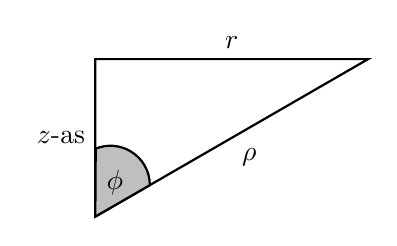
\begin{tikzpicture}[thick]
			\draw(0,0) 
			-- (90:2cm) node[midway,left]{$z$-as} 
			-- (30:4cm) node[midway,above]{$r$} % node of point
			-- (0,0) node[midway,below right]{$\rho$};
			\draw[fill=lightgray, thick] (0,0) 
			-- (30:0.8cm) arc (0:112:0.5cm) node at (60:0.5cm) {$\phi$} 
			 -- cycle;
			
			\end{tikzpicture}
		\end{voorbeeld}
		\subsubsection{Onthoud}
		\begin{tabular}{ll}
			2D: & "$\d A = \d x \d y = r \d r \d \theta$" \\
			3D cilinderco\"ordinaten: & "$\d V = \d x \d y \d z = r \d r \d \theta \d z $" \\
			3D bolco\"ordinaten: & $"=\rho^2 \sin \phi \d \rho \d \phi \d \theta"$
		\end{tabular}
		
		\begin{theorem}[\indx{Bell curve}]
			\[ 
				\int_{-\infty}^{\infty} e^{-x^2} \d x = \sqrt{\pi} \,.
			 \]
		\end{theorem}
		
		\subsection{Stellingen uit het huiswerk}
		\begin{theorem}
			Zij $D,D_1,D_2 \subset \reals^d$ drie Jordanverzamelingen met $D=D_1 \cup D_2$, $D_1 \cap D_2 = \emptyset$. Zij $f$ continu en begrensd op $D$. Dan is $f$ integreerbaar op $D_1$ en $D_2$, en \[ 
				\int_D f = \int_{D_1} f + \int_{D_2} f \,.
			 \]
		\end{theorem}
		
	    
		\newpage
		\section{Tips van Aart}			
		{\bf Belangrijke begrippen analyse 2 week 15.}
\vskip 8pt
\begin{description}
\item[bol, ball] $B(a,r)=\{x\in \mathbb R^d\,|\,|x-a|<r\}$, de open bol rond $a$ met
straal $r$ (in dimensie $d$). $|x-a|$ is de afstand tussen de punten $a$ en $x$,
als $d=1$ is dit hetzelfde als de absolute waarde. Kosmala zou schrijven
$\|\vec x-\vec a\|$.
\item[inwendig punt, interior point] $a\in A$ heet inwendig punt als er een $r>0$ is
met $B(a,r)\subseteq A$ (voor mij zijn $\subseteq$ en $\subset$ gelijkwaardig). Een
inwendig punt behoort noodzakelijk tot de verzameling.
\item[open, inwendige, interior]
$\inw~A$, het inwendige van $A$ is de verzameling inwendige punten van $A$. 
$A$ heet open als
$A=\inw~A$. 
\item[rand, boundary] Punt $a$ heet een randpunt van $A$ als voor elke $r>0$ de bol $B(a,r)$
zowel punten in $A$ als punten niet in $A$ bevat, de rand van $A$ geven we aan met $\partial A$. 
Een randpunt hoeft niet tot de verzameling te behoren.  
\end{description}
{\bf Belangrijke begrippen analyse 2 week 16.}
\vskip 8pt
\begin{description}
\item[verdichtingspunt, accumulation point]
Punt $a$ is {\em verdichtingspunt} van verzameling $A$ als voor alle $r>0$, $B(a,r)$ een punt
van $A$ bevat {\em verschillend} van $a$. $A'$ is de collectie verdichtingspunten. Een 
verdichtingspunt hoeft niet tot de verzameling te behoren.
\item[afsluiting, closure]
De afsluiting $\overline A$ is $A$ samen met zijn verdichtingspunten, het is ook $A$ samen
met zijn rand $\partial A$. $A$ heet gesloten (closed) als hij gelijk is aan zijn afsluiting, dus
als hij al zijn verdichtingspunten bevat, dus als de rand van $A$ in $A$ zit. $A$ is altijd bevat
in zijn afsluiting.
\item[rijen en limieten]
$x^{(n)}\to a$ betekent $\lim_{n\to\infty} x^{(n)}=a$, oftewel:\\ 
voor elke $\epsilon>0$ geldt dat de bol
$B(a,\epsilon)$ voor zekere $N$ alle $x^{(n)}$ bevat waarvoor $n>N$. Oftewel:\\
$\forall\epsilon>0: ~\exists N\in \mathbb N: \forall n>N: |x^{(n)}-a|<\epsilon$. \\
Als de rij $x^{(n)}$ een limiet heeft dan heet de rij {\em convergent}.
\item[infimum en supremum]
Als $A\subset \mathbb R$ niet leeg is en van onderen begrensd, 
dan betekent $m=\inf A$ dat \\
(i) $m\le a$ voor alle $a\in A$; \\
(ii) $m$ is maximaal met betrekking tot eigenschap (i), 
oftewel:\\ 
voor elke $\epsilon>0$ is er een $a\in A$ met $a<m+\epsilon$.\\
Conventies: Als $A$ niet naar beneden begrensd is zeggen ook wel
$\inf A=-\infty$. Als $A=\emptyset$ dan zeggen we ook wel
$\inf A=\infty$.\\ 
Verzin zelf wat $M=\sup A$ betekent.
\end{description}
{\bf Belangrijke begrippen analyse 2 week 17.}
\vskip 8pt
\begin{description}
\item[begrensd, bounded] $A$ heet begrensd als er een $r$ is met $|a|<r$ voor alle
$a\in A$ (dus $A\subseteq B(0,r)$).
\item[(open) overdekking, cover] Een collectie (open) verzamelingen $A_i$, $i\in I$ ($I$ staat 
hier voor een verzameling indices) heet (open) overdekking van $A$ als $A\subseteq \bigcup_{i\in I} A_i$,
dus voor elke $a\in A$ is er een $i\in I$ met $a\in A_i$. Als $J$ een eindige deelverzameling is van
$I$ en als ook $A\subseteq \bigcup_{j\in J} A_j$, dan is dit een eindige deeloverdekking. 
\item[compact] $A$ heet compact als {\em elke} open overdekking van $A$ een eindige deeloverdekking
heeft. Een compacte verzamelingen (in $\mathbb R^d$) is gesloten {\em en} begrensd, dit is `eenvoudig',
omgekeerd is elke gesloten begrensde verzameling compact, dit is niet eenvoudig. `Veel' uitspraken die
waar zijn voor eindige verzamelingen, en onwaar voor willekeurige oneindige verzamelingen, zijn wel waar
voor compacte verzamelingen. 
\end{description}
		{\bf Belangrijke begrippen analyse 2 week 18.}
\vskip 8pt
\begin{description}
\item[limiet] Als $a$ een verdichtingspunt is van $A$, het domein van
de functie $f$, dan betekent $\lim_{x\to a} f(x)=L$:
voor elke $\epsilon>0$ is er een $\delta>0$ zodat als 
$x\in A\setminus\{a\}$ en $|x-a|<\delta$, 
dan $|f(x)-L|<\epsilon$.
\item[hoogtelijnen] Voor level curves: aarzel niet Mathematica te gebruiken.
\item[tip limieten] Voor limieten: probeer zoveel mogelijk de insluitstelling
te gebruiken. Ook Taylorreeksen zijn vaak nuttig.
\item[Som Kosmala] 10.2.9: onderscheid de gevallen $x\ne y$ en $x=y$.
\end{description}
\vskip 8pt
{\bf Belangrijke begrippen analyse 2 week 19.}
\begin{description}
\item[Uniform continu] Voor elke $\epsilon>0$ is er
een $\delta>0$ zodanig dat voor elke $a$ en $b$ in het domein van $f$ 
geldt $|f(a)-f(b)|<\epsilon$ als $|a-b|<\delta$.
\item[Banach] Als $f\,:\,D\to D(\subset \mathbb R^d)$ een contractie
is en $D$ gesloten, dan is er een uniek vast punt $p$ (dus waarvoor $f(p)=p$), en voor elke
$x\in D$ convergeert de rij $x,f(x),f(f(x)),\dots$ naar dit punt $p$. \\
$f$ heet contractie op $D$ als er een $q<1$ is met $|f(x)-f(y)|\le q|x-y|$
voor alle $x,y\in D$.
\end{description}
\vskip 8pt
{\bf Belangrijke begrippen analyse 2 week 20.}
\begin{description}
\item[Parti\"ele afgeleiden] $\ds \partial_xf(a,b)=\lim_{h\to 0}\frac{f(a+h,b)-f(a,b)}h$.
Iets dergelijks voor $\partial_y$ en voor functies van (nog) meer variabelen.
Beetje verwarrend: met $\partial_{xy}f$ of ook $f_{xy}$ bedoelen we $\partial_y(\partial_xf)$,
we differentieren hier dus {\em eerst} naar $x$ en dan naar $y$ (voor {\em fatsoenlijke}
functies maakt de volgorde overigens niet uit).
\item[Differentieerbaar] $f\,:\,\mathbb R^2\to\mathbb R$ is differentieerbaar in $(a,b)$
als er getallen $m_1$ en $m_2$ zijn met 
$f(a+h,b+k)=f(a,b)+m_1h+m_2k+\epsilon\sqrt{h^2+k^2}$ waarbij $\epsilon\to0$ als $(h,k)\to(0,0)$.
hier zijn $m_1$ en $m_2$ de parti\"ele afgeleiden $\partial_xf(a,b)$ en $\partial_y$. 
Het beginstuk heet de linearisering van $f$ rond $(a,b)$ en geeft de vergelijking van het
raakvlak. Iets dergelijks voor meer variabelen.
\end{description}
		
{\bf Belangrijke begrippen analyse 2 week 22.}
\vskip 8pt
\begin{description}
\item[Jacobiaan] Als $(f_1,f_2,\dots,f_n)=f\,:\,\mathbb R^d\to \mathbb R^n$ differentieerbaar is
in het punt $a=(a_1,\dots,a_d)$ dan wordt de afgeleide $Df(a)$ gegeven
door de ($n\times d$) Jacobiaan $M_{ij}=\partial_jf_i(a)$. Er geldt $f(a+h)=f(a)+Mh+\epsilon\|h\|$,
waar $\epsilon$ een vector is met limiet $\bf 0$ als $\|h\|\to 0$.
\item[Kettingregel] Als $x(t),y(t)\,:\,\mathbb R\to\mathbb R$ en $f(x,y)\,:\,\mathbb R^2\to R$
en $z=f(x(t),y(t))$ 
\[
\frac{dz}{dt}=\frac{\partial f}{\partial x}\frac{dx}{dt}+\frac{\partial f}{\partial y}\frac{dy}{dt}.
\]
Als $x(t,s),y(t,s)\,:\,\mathbb R^2\to\mathbb R^2$ en $z=f(x,y)$ dan
\[
\frac{\partial z}{\partial t}=\frac{\partial z}{\partial x}\frac{\partial x}{\partial t}
+\frac{\partial z}{\partial y}\frac{\partial y}{\partial t}.
\]
\item[Taylor (rond 0), drie variabelen] $f(x,y,z)\,:\,\mathbb R^3\to \mathbb R$:
\[
\!\!\!\!\!\!\!\!\!\!\!\!\!\!\!\!\!\!\!\! T(h,k,l)=f({\bf 0})+ f_x({\bf 0})h + f_y k+ f_z l+
\frac12 f_{xx}h^2+ f_{xy}hk +\cdots+\frac16 f_{xxx}h^3+\frac12 f_{xxy}h^2k+ f_{xyz}hkl +\cdots. 
\] 
\end{description}
\vskip 8pt
{\bf Belangrijk begrip analyse 2 week 23.}
\begin{description}
\item[Impliciete functiestelling] $F\,:\,D\to \mathbb R^m$ met
$(x_0,y_0)\in D\subset \mathbb R^n\times \mathbb R^m$ en $F(x_0,y_0)=0$
en $D_yF(x_0,*)$ inverteerbaar in $*=y_0$, dan zijn er open $U\ni (x_0,y_0)$ en
$V\ni x_0$ en differentieerbare b $g\,:\,V\to\mathbb R^m$, met\\
(i) $x\in V$, $y\in\mathbb R^m: y=g(x) \Leftrightarrow ((x,y)\in U\wedge F(x,y)=0)$.\\
(ii) $x\in V$: $Dg(x)=-[D_yF(x,g(x))]^{-1}D_xF(x,y)$.\\[6pt]  
Dus hier zijn $D_yF(x,*)$ en $D_xF(*,y)$ de Jacobianen van de afbeeldingen
$F(x,*)\,:\,\mathbb R^m\to\mathbb R^m$ en $F(*,y)\,:\,\mathbb R^n\to \mathbb R^m$,
dus $D_y$ is een $m\times m$ matrix en $D_x$ is een $m\times n$ matrix. 

\end{description}
		
		\newpage
		
		\appendix
		\section{Appendix: LaTeX tips}
		
		\opm Deze tips hebben deels betrekking op de hier gebruikte macro's.
		
		\subsection{Beste allemaal}
		
		Mijn complimenten -- dit is de eerste keer dat ``m'n'' studenten alle lecture notes in \LaTeX typen.
		Prima job!
		
		\ \\
		Ik heb in het \verb$.tex$ bestand definities toegevoegd -- geen aktie noodzakelijk -- tussen
		``start nieuwe macros'' en ``einde nieuwe macros'' die het
		typewerk sterk kunnen vergemakkelijken. ``Makkelijk'' is smaakafhankelijk.
		
		\ \\
		Ik stel voor -- maar dat hoeft vanzelfsprekend niet -- dat ``jullie'' de typografie aanpassen aan wat in de Analyse/Calculus gebruikelijk is -- een deel heb ik al als voorbeeld voorgedaan in de brontekst van dit bestand:
		\begin{itemize}
			\item In plaats van de letter x, y en z \textbf{die vectoren zijn in dit} \verb$.tex$ \textbf{bestand}, type
			\verb$\x$, \verb$\y$ en \verb$\z$: $\x, \y, \z$
			\item Voor alle vectoren zoals $\mathbf{a}$, $\mathbf{b}$ etc: Type \verb$\a$, \verb$\b$, etc
			%\item Ditto voor vectorwaardige functies \verb$\f\:\reals^d\to\reals$: $\f\:\reals^d\to\reals$: Type \verb$\f$
			%% Author's note (Thomas): Don't agree, see for example http://tex.stackexchange.com/questions/5170/mapsto-vs-rightarrow
			\item In plaats van de letter 0 type voor nulvectoren \verb$\zero$: $\zero$
			\item In plaats van \verb$|x|$ type \verb$\abs{x}$: $\abs{x}$
			\item In plaats van \verb$|\x|$ type \verb$\abs{\x}$: $\abs{\x}$
			\item In plaats van \verb$x^{(n)}$ type \verb$x\up{n}$: $x\up{n}$
			\item In plaats van \verb$\x^{(n)}$ type \verb$\x\up{n}$: $\x\up{n}$
			\item In plaats van \verb$\iff$ type \verb$\iff$: $\iff$
			\item In plaats van \verb$\implies$ type \verb$\implies$: $\implies$
			\item In plaats van \verb$\mathbb{R}$ type \verb$\reals$: $\reals$ (heb ik al vervangen)
			\item In plaats van \verb$\mathbb{N}$ type \verb$\naturals$: $\naturals$ (heb ik al vervangen)
			\item In plaats van \verb$:$ type \verb$\:$: $x\: y$
			\item Voor verzamelingen type bv \verb$\set{1,2,3}$: $\set{1,2,3}$
			\item Voor rode tekst gebruik \verb$\red{word 1 and 2}$ type \verb$\red{word 1 and 2}$: \red{word 1 and 2}
			\item Voor groene tekst gebruik \verb$\grn{word 1 and 2}$ type \verb$\grn{word 1 and 2}$: \grn{word 1 and 2}
			\item Voor blauwe tekst gebruik \verb$\blu{word 1 and 2}$ type \verb$\blu{word 1 and 2}$: \blu{word 1 and 2}
			\item \blu{Het} \verb$\blu{...}$ \blu{kleuren commando kan geen} \verb#\verb$...$# \blu{constructie bevatten.}
			\item De langere variant \verb$\{\color{blue}...}$ kan wel \verb#\verb$...$# in de \dots bevatten!
			\item De langere variant \verb$\{\color{red}...}$ kan wel \verb#\verb$...$# in de \dots bevatten!
			\item De langere variant \verb$\{\color{green}...}$ kan wel \verb#\verb$...$# in de \dots bevatten!
			\item In plaats van \verb$\define$ type \verb$\begin{define}[onderwerp] ..... \end{define}$: zie voorbeelden in dit \verb$.tex$ bestand
			\item Om een \verb$woord$ in de index te plaatsen, type \verb$\indx{woord}$ -- het verschijnt dan ``slanted'' in de \verb$.pdf$
			\item In \LaTeX\ zijn de braces \verb${...}$ de \LaTeX\ groep-open en \LaTeX\ groep-sluit operatoren -- en daarom niet zichtbaar in de tekst. Om ze zichtbaar te maken moet je \verb$\lbrace$ resp.{} \verb$\rbrace$ typen of -- minder slim als je \LaTeX\ beter kent type je \verb$\{$ resp.{} \verb$\}$.
			\item Als je zulke braces (\verb$\{\}$, \verb$()$, \verb$[]$) groot genoeg wilt hebben dan type je \verb$\left\lbrace ... \right\rbrace$:
			\[
			\left\lbrace \int_0^1 f(x) \text{d}x \right\rbrace.
			\]
			Een minder alternatief -- alleen te snappen met meer \LaTeX\ kennis is \verb$\big\{$ ipv.{} \verb$\left\rbrace$.
			\item Als je in het \verb$.pdf$ wilt kunnen klikken op secties om daarnaar toe te springen includeer dan
			\verb$\usepackage{hyperref}$ -- heb ik al gedaan -- dit package was al wel geincludeerd maar het automatisch springen was uitgeschakeld.
			\item De definities van \verb$\intr$ en \verb$\distr$ heb ik aangepast -- dat valt niet op maar daar komt later voordeel van
			\item De \verb$\AA$ geeft niet de gewenst ``interior'' notatie -- daarom heb ik \verb$\AA$ aangepast aan de \LaTeX\ standaard
			om $\mathring{A}$ te geven
			\item In plaats van \verb$\lim_{n\to\infty}$ type de kortere \LaTeX\ standaard \verb$\lim_{n\to\infty}$: $\lim_{n\to\infty}$
			\item De bold -- vetgedrukte -- vectoren veranderen in underline vectoren door 1 regel te wijzigen!
			\item In math mode -- tussen dollars en \verb$\[\]$ gebruik \verb$\ldots$ voor enumeraties zoals \verb$1,2,\ldots,d$: $1,2,\ldots,d$ -- gebruik \verb$\dots$ alleen in text mode, of bij enumeraties met symbolen zoals $+$ of $<$: \verb$1+2+\dots+d$: $1+2+\dots+d$. 
		\end{itemize}
		Ik stel voor dat jullie deze tips verhuizen naar de appendix voor de volgende generatie -- die appendix heb ik toegevoegd.
		
		\ \\
		Groet,
		
		Jos.
		
		\phantomsection
%		\newpage
%		\bibliographystyle{plain}
%		\addcontentsline{toc}{chapter}{Bibliography}\bibliography{orgcite}
		\newpage
		\addcontentsline{toc}{chapter}{Index} 
%		\begin{scriptsize}
			\printindex
%		\end{scriptsize}
		
\end{document} 
